\documentclass[]{article}
\usepackage{lmodern}
\usepackage{unicode-math}
\usepackage{amssymb,amsmath}
\usepackage{ifxetex,ifluatex}
\usepackage{fixltx2e} % provides \textsubscript
\ifnum 0\ifxetex 1\fi\ifluatex 1\fi=0 % if pdftex
  \usepackage[T1]{fontenc}
  \usepackage[utf8]{inputenc}
\else % if luatex or xelatex
  \ifxetex
    \usepackage{mathspec}
    \usepackage{xltxtra,xunicode}
  \else
    \usepackage{fontspec}
  \fi
  \defaultfontfeatures{Mapping=tex-text,Scale=MatchLowercase}
  \newcommand{\euro}{€}
\fi
% use upquote if available, for straight quotes in verbatim environments
\IfFileExists{upquote.sty}{\usepackage{upquote}}{}
% use microtype if available
\IfFileExists{microtype.sty}{\usepackage{microtype}}{}
\usepackage{graphicx}
\makeatletter
\def\maxwidth{\ifdim\Gin@nat@width>\linewidth\linewidth\else\Gin@nat@width\fi}
\def\maxheight{\ifdim\Gin@nat@height>\textheight\textheight\else\Gin@nat@height\fi}
\makeatother
% Scale images if necessary, so that they will not overflow the page
% margins by default, and it is still possible to overwrite the defaults
% using explicit options in \includegraphics[width, height, ...]{}
\setkeys{Gin}{width=\maxwidth,height=\maxheight,keepaspectratio}
\ifxetex
  \usepackage[setpagesize=false, % page size defined by xetex
              unicode=false, % unicode breaks when used with xetex
              xetex]{hyperref}
\else
  \usepackage[unicode=true]{hyperref}
\fi
\hypersetup{breaklinks=true,
            bookmarks=true,
            pdfauthor={},
            pdftitle={},
            colorlinks=true,
            citecolor=blue,
            urlcolor=blue,
            linkcolor=magenta,
            pdfborder={0 0 0}}
\urlstyle{same}  % don't use monospace font for urls
\setlength{\parindent}{0pt}
\setlength{\parskip}{6pt plus 2pt minus 1pt}
\setlength{\emergencystretch}{3em}  % prevent overfull lines
\setcounter{secnumdepth}{0}


\begin{document}

\section{Abstract}\label{abstract}

Machine learning is a growing area in computer science. Neural networks
is very popular subdomain of it. This project generally covers the work
of M. Nielsen and his book Neural Networks and Deep Learning{[}1{]}. We
will first introduce neual networks and then aplly it to a generic
problem which is called classifying handwritten digits.

\section{Introduction}\label{introduction}

The idea of neural networks is to take a large number of dataset known
as training examples, and then develop a system which can learn from
those training examples. In other words, the neural network uses the
examples to automatically infer rules for recognizing other unknown
examples. Furthermore, by increasing the number of training examples,
the network can learn more about handwriting, and so improve its
accuracy.

There are just 100 training digits below, perhaps we could build a
better handwriting recognizer by using thousands or even millions or
billions of training examples.

\begin{figure}[htbp]
\centering
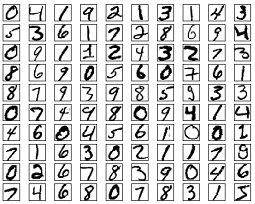
\includegraphics{http://neuralnetworksanddeeplearning.com/images/mnist_100_digits.png}
\caption{100\_handwritten\_digits}
\end{figure}

This project is concerned with write a computer program implementing a
neural network that learns to recognize handwritten digits.

Along the way there are many key ideas about neural networks, including
two important types of artificial neuron (the perceptron and the sigmoid
neuron), and the standard learning algorithm for neural networks, known
as stochastic gradient descent.

\subsection{Perceptrons}\label{perceptrons}

Perceptron is a type of artificial neuron. Perceptrons were developed in
the 1950s and 1960s by the scientist Frank Rosenblatt, inspired by
earlier work by Warren McCulloch and Walter Pitts. Today, it's more
common to use other models of artificial neurons - in this book, and in
much modern work on neural networks, the main neuron model used is one
called the sigmoid neuron.

A perceptron takes several binary inputs, $ x\_1, x\_2, \ldots{}, $
and produces a single binary output:

\begin{figure}[htbp]
\centering
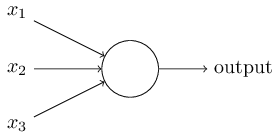
\includegraphics{http://neuralnetworksanddeeplearning.com/images/tikz0.png}
\caption{binary\_inputs}
\end{figure}

In general it could have more or fewer inputs. Rosenblatt proposed a
simple rule to compute the output. He introduced weights,
w1,w2,\ldots{}, real numbers expressing the importance of the respective
inputs to the output. The neuron's output, 0 or 1, is determined by
whether the weighted sum $ \sum\emph{j w}jx\_j $ is less than or
greater than some threshold value. Just like the weights, the threshold
is a real number which is a parameter of the neuron. To put it in more
precise algebraic terms:

\begin{equation}
        output =
        \begin{cases}
            0,& if \hspace{0.5 cm} \sum_j\ w_jx_j \leqslant threshold \\
            1,& if \hspace{0.5 cm} \sum_j\ w_jx_j > threshold
        \end{cases}
\end{equation}

That's all there is to how a perceptron works!

That's the basic mathematical model. A way you can think about the
perceptron is that it's a device that makes decisions by weighing up
evidence.

Obviously, the perceptron isn't a complete model of human
decision-making! But what the example illustrates is how a perceptron
can weigh up different kinds of evidence in order to make decisions. And
it should seem plausible that a complex network of perceptrons could
make quite subtle decisions:

\begin{figure}[htbp]
\centering
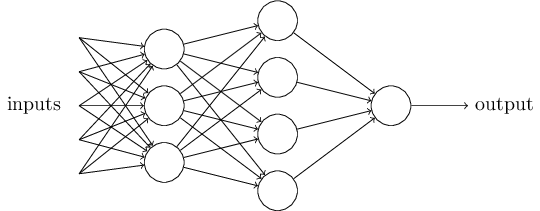
\includegraphics{http://neuralnetworksanddeeplearning.com/images/tikz1.png}
\caption{complex\_network}
\end{figure}

In this network, the first column of perceptrons - the first layer of
perceptrons - is making three very simple decisions, by weighing the
input evidence. What about the perceptrons in the second layer? Each of
those perceptrons is making a decision by weighing up the results from
the first layer of decision-making. In this way a perceptron in the
second layer can make a decision at a more complex and more abstract
level than perceptrons in the first layer. And even more complex
decisions can be made by the perceptron in the third layer. In this way,
a many-layer network of perceptrons can engage in sophisticated decision
making.

In the first example, it is defined perceptrons has just a single
output. In the network above the perceptrons look like they have
multiple outputs. In fact, they're still single output. The multiple
output arrows are merely a useful way of indicating that the output from
a perceptron is being used as the input to several other perceptrons.
It's less unwieldy than drawing a single output line which then splits.

Let's simplify the way we describe perceptrons. The first change is to
write $ \sum\emph{j w}jx\_j $ as a dot product,
$ w \cdot x \equiv \sum\emph{j w}jx\_j $ ,
where w and x are vectors whose components are the weights and inputs, respectively.
The second change is to move the threshold to the other side of the inequality, and to replace
it by what's known as the perceptron's bias, $ b \equiv −threshold. $ Using the bias instead of the threshold, the
perceptron rule can be rewritten:

\begin{equation}
    output =
    \begin{cases}
        0,& if  \hspace{0.5 cm} w \cdot x + b \leq 0 \\
        1,& if  \hspace{0.5 cm}  w \cdot x + b > 0
    \end{cases}
\end{equation}

You can think of the bias as a measure of how easy it is to get the
perceptron to output a 1. Or to put it in more biological terms, the
bias is a measure of how easy it is to get the perceptron to fire. For a
perceptron with a really big bias, it's extremely easy for the
perceptron to output a 1. But if the bias is very negative, then it's
difficult for the perceptron to output a 1.

\subsection{Sigmoid neurons}\label{sigmoid-neurons}

Suppose we have a network of perceptrons that we'd like to use to learn
to solve some problem. For example, the inputs to the network might be
the raw pixel data from a scanned, handwritten image of a digit. And
we'd like the network to learn weights and biases so that the output
from the network correctly classifies the digit. To see how learning
might work, suppose we make a small change in some weight (or bias) in
the network. What we'd like is for this small change in weight to cause
only a small corresponding change in the output from the network. As
we'll see in a moment, this property will make learning possible.
Schematically, here's what we want (obviously this network is too simple
to do handwriting recognition!):

\begin{figure}[htbp]
\centering
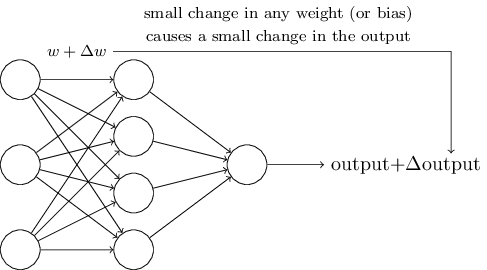
\includegraphics{http://neuralnetworksanddeeplearning.com/images/tikz8.png}
\caption{weight\_small\_change}
\end{figure}

If it were true that a small change in a weight (or bias) causes only a
small change in output, then we could use this fact to modify the
weights and biases to get our network to behave more in the manner we
want.

The problem is that this isn't what happens when our network contains
perceptrons. In fact, a small change in the weights or bias of any
single perceptron in the network can sometimes cause the output of that
perceptron to completely flip, say from 0 to 1. That flip may then cause
the behaviour of the rest of the network to completely change in some
very complicated way.

We can overcome this problem by introducing a new type of artificial
neuron called a sigmoid neuron. Sigmoid neurons are similar to
perceptrons, but modified so that small changes in their weights and
bias cause only a small change in their output. That's the crucial fact
which will allow a network of sigmoid neurons to learn.

Okay, let me describe the sigmoid neuron. We'll depict sigmoid neurons
in the same way we depicted perceptrons. Just like a perceptron, the
sigmoid neuron has inputs, $ x\_1, x\_2, \ldots{} $ But instead of
being just 0 or 1, these inputs can also take on any values between 0
and 1. So, for instance, 0.638\ldots{} is a valid input for a sigmoid
neuron. Also just like a perceptron, the sigmoid neuron has weights for
each input, $ w\_1, w\_2, \ldots{} $ and an overall bias, $ b
$. But the output is not 0 or 1. Instead, it's $ \sigma (w \cdot x + b) $,
where $ \sigma $ is called the sigmoid function - sometimes called
logistic function - and this new class of neurons called sigmoid neurons
or logistic neurons. and is defined by:

\begin{equation}
    \sigma(z) \equiv \frac{1}{1 + e^{-z}}
\end{equation}

The output of a sigmoid neuron with inputs $ x\_1, x\_2, \ldots{} $
weights $ w\_1, w\_2, \ldots{} $ and bias $ b $ is

\begin{equation}
    \frac {1}{1+exp(−\sum_j w_jx_j − b)}
\end{equation}

To understand the similarity to the perceptron model, suppose $ z
\equiv w \cdot x + b $ is a large positive number. Then $ e \^{}
\{−z\} \approx 0 $ and so $ \sigma(z) \approx 1 $ just as it would
have been for a perceptron. Suppose on the other hand that $ z = w
\cdot x + b $ is very negative. Then $ e \^{} \{−z\}
\to \infty $, and $ \sigma(z) \approx 0 $ like a perceptron. The shape
is:

\begin{figure}[htbp]
\centering
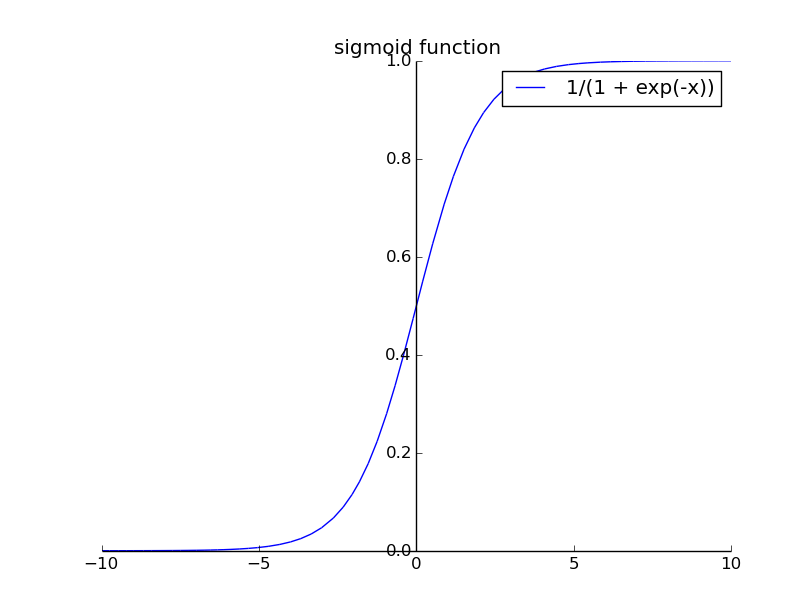
\includegraphics{https://lh3.googleusercontent.com/-WNMDpgwcC7I/VYk-QEgs9DI/AAAAAAAAAT8/MKuAMcVDYcM/s0/sigmoid_function.png}
\caption{sigmoid\_function}
\end{figure}

This shape is a smoothed out version of a step function or Heaviside
step function:

\begin{figure}[htbp]
\centering
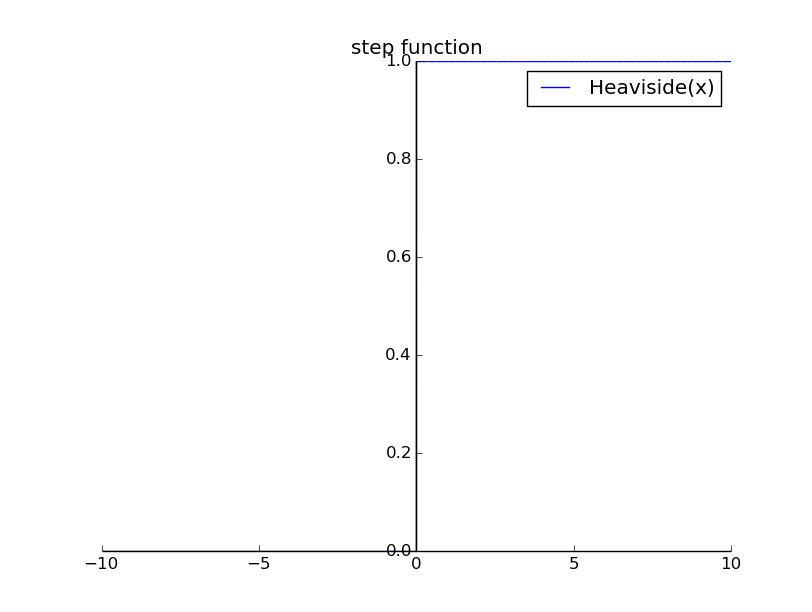
\includegraphics{https://lh3.googleusercontent.com/-lIMAxDaKs5U/VYlCQHeg_1I/AAAAAAAAAUM/gQwIY5OWpAo/s0/step_function.png}
\caption{step\_function}
\end{figure}

If $ \sigma $ had in fact been a step function, then the sigmoid
neuron would be a perceptron, since the output would be 1 or 0 depending
on whether $ w \cdot x + b $ was positive or negative. Actually, when
$ w \cdot x + b = 0 $ the perceptron outputs 0, while the step
function outputs 1. So, strictly speaking, we would need to modify the
step function at that one point.

By using the actual $ \sigma $ function we get, a smoothed out
perceptron. The smoothness of $ \sigma $ means that small changes $
\Delta w\_j $ in the weights and $ \Delta b $ in the bias will
produce a small change $ \Delta output $ in the output from the
neuron. In fact, calculus tells us that $ \Delta output $ is well
approximated by

\begin{equation}
    \Delta output \approx \sum_j
    \frac {\partial \ output}{\partial w_j} \Delta w_j +
    \frac {\partial \ output}{\partial b} \Delta b
\end{equation}

where the sum is over all the weights, $ w\_j $, and $
\frac{\partial \ output}{\partial w_j} $ and $
\frac{\partial \ output}{\partial b} $ denote partial derivatives of
the output with respect to $ w\_j $ and $ b $, respectively. So
while sigmoid neurons have much of the same qualitative behaviour as
perceptrons, they make it much easier to figure out how changing the
weights and biases will change the output.

If it's the shape of $ \sigma $ which really matters, and not its
exact form, then why use the particular form used for $ \sigma $ ? In
fact, there are other activation functions as well. The main thing that
changes when we use a different activation function is that the
particular values for the partial derivatives in Equation (5) change. It
turns out that when we compute those partial derivatives, using $
\sigma $ will simplify the algebra.

\begin{equation}
    \begin{split}
        \frac{d\sigma}{dz} &= \left({1 - \frac{1}{1 + e ^ {-z}}}\right)
        \left(\frac{1}{1 + e ^ {-z}}\right)\\
        &=(1 - \sigma)\sigma
    \end{split}
\end{equation}

\subsection{The architecture of neural
networks}\label{the-architecture-of-neural-networks}

Suppose we have the network:

\begin{figure}[htbp]
\centering
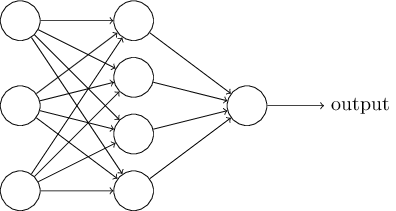
\includegraphics{http://neuralnetworksanddeeplearning.com/images/tikz10.png}
\caption{architecture}
\end{figure}

As mentioned earlier, the leftmost layer in this network is called the
input layer, and the neurons within the layer are called input neurons.
The rightmost or output layer contains the output neurons, or, as in
this case, a single output neuron. The middle layer is called a hidden
layer, since the neurons in this layer are neither inputs nor outputs.
The network above has just a single hidden layer, but some networks have
multiple hidden layers. For example, the following four-layer network
has two hidden layers:

\begin{figure}[htbp]
\centering
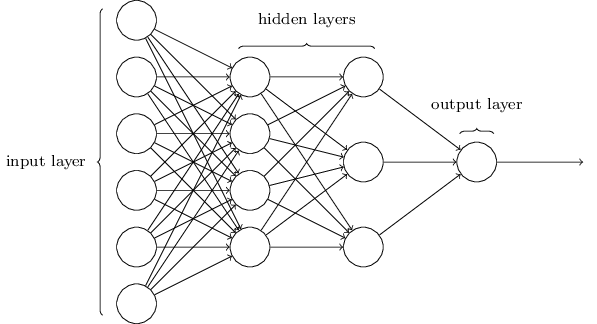
\includegraphics{http://neuralnetworksanddeeplearning.com/images/tikz11.png}
\caption{two\_hidden\_layers}
\end{figure}

Somewhat confusingly, and for historical reasons, such multiple layer
networks are sometimes called multilayer perceptrons or MLPs, despite
being made up of sigmoid neurons, not perceptrons. It is not going to be
used the MLP terminology in this book, since it is confusing.

There can be quite an art to the design of the hidden layers. Neural
networks researchers have developed many design heuristics for the
hidden layers, which help people get the behaviour they want out of
their nets. For example, such heuristics can be used to help determine
how to trade off the number of hidden layers against the time required
to train the network.

Up to now, we've been discussing neural networks where the output from
one layer is used as input to the next layer. Such networks are called
feedforward neural networks. This means there are no loops in the
network - no feedback-. Loops would be problematic in for example
sigmoid neurons because of the inputs would depend on the outputs.
However, there are other models of artificial neural networks in which
feedback loops are possible. These models are called recurrent neural
networks. The idea in these models is to have neurons which fire for
some limited duration of time, before becoming quiescent. That firing
can stimulate other neurons, which may fire a little while later, also
for a limited duration. That causes still more neurons to fire, and so
over time we get a cascade of neurons firing. Loops don't cause problems
in such a model, since a neuron's output only affects its input at some
later time, not instantaneously.

Recurrent neural nets have been less influential than feedforward
networks, in part because the learning algorithms for recurrent nets are
(at least to date) less powerful. But recurrent networks are still
extremely interesting. They're much closer in spirit to how our brains
work than feedforward networks. And it's possible that recurrent
networks can solve important problems which can only be solved with
great difficulty by feedforward networks.

\subsection{A simple network to classify handwritten
digits}\label{a-simple-network-to-classify-handwritten-digits}

We can split the problem of recognizing handwritten digits into two
sub-problems. First, we'd like a way of breaking an image containing
many digits into a sequence of separate images, each containing a single
digit.

\begin{figure}[htbp]
\centering
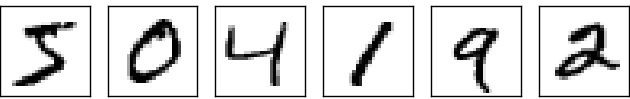
\includegraphics{http://neuralnetworksanddeeplearning.com/images/digits_separate.png}
\caption{digits\_sequence}
\end{figure}

Once the image has been segmented, the program then needs to classify
each individual digit. We will focus on writing a program to classify
individual digits..

To recognize individual digits we will use a three-layer neural network:

\begin{figure}[htbp]
\centering
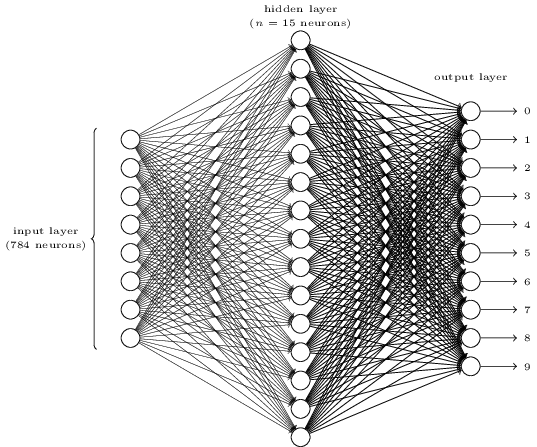
\includegraphics{http://neuralnetworksanddeeplearning.com/images/tikz12.png}
\caption{three\_layer\_neural\_net}
\end{figure}

As discussed in the next section, our training data for the network will
consist of many 28 by 28 pixel images of scanned handwritten digts, and
so the input layer contains $ 784 = 28 \times 28 $ neurons. The input
pixels are grayscale, with a value of 0.0 representing white, a value of
1.0 representing black, and in between values representing gradually
darkening shades of grey.

The second layer of the network is a hidden layer. We denote the number
of neurons in this hidden layer by n, and we'll experiment with
different values for n.

Why we use 10 output neurons. After all, the goal of the network is to
tell us which digit $ (0, 1, 2, \ldots{}, 9) $ corresponds to the
input image. A seemingly natural way of doing that is to use just 4
output neurons, treating each neuron as taking on a binary value,
depending on whether the neuron's output is closer to 0 or to 1. Four
neurons are enough to encode the answer, since $ 2 \^{} 4 = 16 $ is
more than 10 possible values for the input digit. Why should our network
use 10 neurons instead? The ultimate justification is empirical. We can
try out both network designs, and it turns out that, for this particular
problem, the network with 10 output neurons learns to recognize digits
better than the network with 4 output neurons. But that leaves us
wondering why using 10 output neurons works better?

\begin{figure}[htbp]
\centering
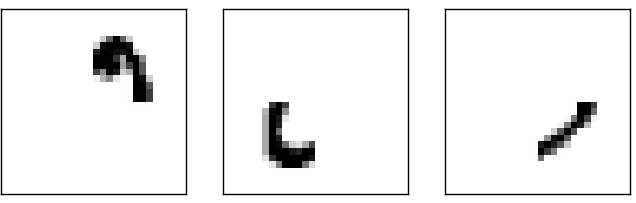
\includegraphics{http://neuralnetworksanddeeplearning.com/images/mnist_other_features.png}
\caption{0shapes}
\end{figure}

First neuron in the hidden layer may detect just whether or not an image
like the above is present. If we had 4 outputs, then the first output
neuron would be trying to decide what the most significant bit of the
digit was. And there's no easy way to relate that most significant bit
to simple shapes like those shown above. However there could be always
such structures with 4 neurons at the output so that net were more
efficient. Now, with all that said, this is all just a heuristic.

\subsection{Learning with gradient
descent}\label{learning-with-gradient-descent}

Now the first thing we'll need is a data set to learn from so-called
training data set. We'll use the
\href{http://yann.lecun.com/exdb/mnist/}{MNIST data set} which contains
tens of thousands of scanned images of handwritten digits, together with
their correct classifications. Images are the same as used before.

\begin{figure}[htbp]
\centering
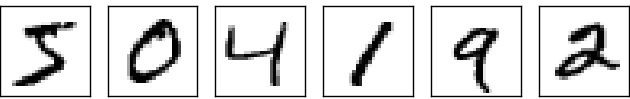
\includegraphics{http://neuralnetworksanddeeplearning.com/images/digits_separate.png}
\caption{MNIST}
\end{figure}

The MNIST data comes in two parts. The first part contains 60,000 images
to be used as training data. These images are scanned handwriting
samples from 250 people, half of whom were US Census Bureau employees,
and half of whom were high school students. The images are grayscale and
28 by 28 pixels in size. The second part of the MNIST data set is 10,000
images to be used as test data. Again, these are 28 by 28 grayscale
images. We'll use the test data to evaluate how well our neural network
has learned to recognize digits. To make this a good test of
performance, the test data was taken from a different set of 250 people
than the original training data (albeit still a group split between
Census Bureau employees and high school students). This helps give us
confidence that our system can recognize digits from people whose
writing it didn't see during training.

We'll use the notation $ x $ to denote a training input. It'll be
convenient to regard each training input $ x $ as a $ 28 \times 28 =
784 $ dimensional vector. Each entry in the vector represents the gray
value for a single pixel in the image. We'll denote the corresponding
desired output by $ y = y(x) $, where $ y $ is a 10-dimensional
vector. For example, if a particular training image, $ x
$, depicts a 6, then $ y(x)=(0,0,0,0,0,0,1,0,0,0) \^{} T $ is the
desired output from the network. Note that $ T $ here is the transpose
operation, turning a row vector into an ordinary (column) vector.

What we'd like is an algorithm which lets us find weights and biases so
that the output from the network approximates $ y(x) $ for all
training inputs $ x $. To quantify how well we're achieving this goal
we define a cost function. Sometimes referred to as a loss or objective
function.

\begin{equation}
    C(w, \ b)\equiv\frac{1}{2n}\sum_x ||y(x) − a||^2
\end{equation}

Here, $ w $ denotes the collection of all weights in the network, $ b
$ all the biases, $ n $ is the total number of training inputs, $ a
$ is the vector of outputs from the network when $ x $ is input, and
the sum is over all training inputs, x. Of course, the output $ a $
depends on $ x, w $ and $ b $. The notation $
\textbar{}\textbar{}v\textbar{}\textbar{} $ just denotes the usual
length function for a vector $ v $. We'll call $ C $ the quadratic
cost function; it's also sometimes known as the mean squared error or
just MSE. $ C(w, ~b) $ is non-negative, since every term in the sum is
non-negative. Furthermore, the cost $ C(w, ~b) $ precisely when $
y(x) $ is approximately equal to the output, $ a
$, for all training inputs, $ x
$. So our training algorithm has done a good job if it can find weights and biases so that $
C(w, ~b) \approx 0 $. By contrast, it's not doing so well when $ C(w,
~b) $ is large - that would mean that $ y(x) $ is not close to the
output a for a large number of inputs. So the aim of our training
algorithm will be to minimize the cost $ C(w, ~b) $ as a function of
the weights and biases.

Okay, let's suppose we're trying to minimize some function, $ C(v)
$. This could be any real-valued function of many variables, $ v = v1,
v2, \ldots{} $

\begin{figure}[htbp]
\centering
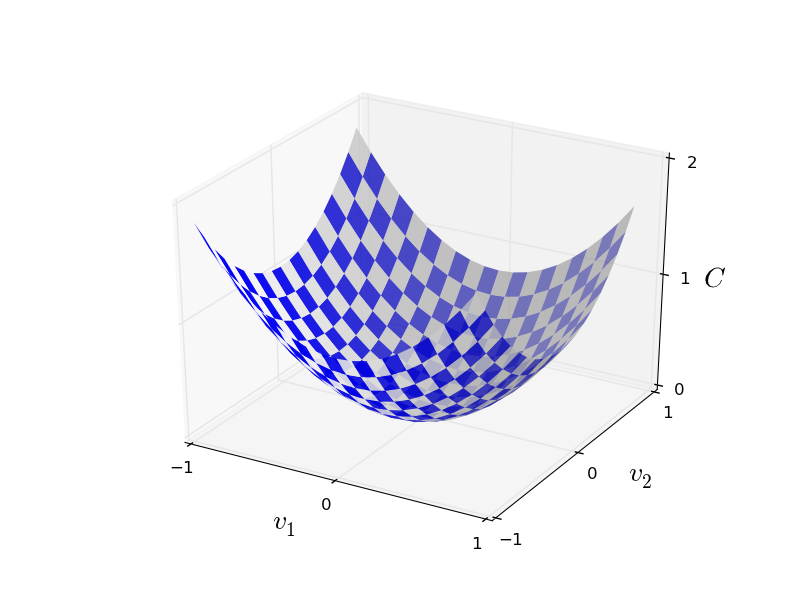
\includegraphics{http://neuralnetworksanddeeplearning.com/images/valley.png}
\caption{valley}
\end{figure}

What we'd like is to find where $ C $ achieves its global minimum. One
way of attacking the problem is to use calculus to try to find the
minimum analytically. With some luck that might work when $ C $ is a
function of just one or a few variables. But it'll turn into a nightmare
when we have many more variables. And for neural networks we'll often
want far more variables - the biggest neural networks have cost
functions which depend on billions of weights and biases in an extremely
complicated way. Using calculus to minimize that just won't work! We
start by thinking of our function as a kind of a valley. And we imagine
a ball rolling down the slope of the valley. Our everyday experience
tells us that the ball will eventually roll to the bottom of the valley.

Let's think about what happens when we move the ball a small amount $
\Delta v\_1 $ in the $ v\_1 $ direction, and a small amount $
\Delta v\_2 $ in the $ v\_2 $ direction. Calculus tells us that C
changes as follows:

\begin{equation}
    \Delta C \approx \frac {\partial C}{\partial v_1} \Delta v_1 +
    \frac{\partial C}{\partial v_2} \Delta v_2
\end{equation}

We're going to find a way of choosing $ \Delta v\_1 $ and $
\Delta v\_2 $ so as to make $ \Delta C $ negative; i.e., we'll choose
them so the ball is rolling down into the valley. To figure out how to
make such a choice it helps to define $ \Delta v $ to be the vector of
changes in $ v $, $ \Delta v \equiv (\Delta v\_1, ~\Delta v\_2)\^{}T
$. We denote the gradient vector by $ \nabla C $, i.e.:

\begin{equation}
    \nabla C \equiv \left( \frac{\partial C}{\partial v_1}, \ \frac{\partial C}
    {\partial v_2} \right)^T
\end{equation}

More generally, if $ C $ is function of $ m $ variables,

\begin{equation}
    \nabla C \equiv \left( \frac{\partial C}{\partial v_1},
    \frac{\partial C}{\partial v_2}, \ ..., \ \frac{\partial C}
    {\partial v_m} \right)^T
\end{equation}

With these definitions, the expression (8) for $ \Delta C $ can be
rewritten as

\begin{equation}
    \Delta C \approx \nabla C ⋅ \Delta v
\end{equation}

In particular, suppose we choose,

\begin{equation}
    \Delta v = −\eta \nabla C
\end{equation}

where $ \eta $ is a small, positive parameter (known as the learning
rate). Then Equation (11) becomes

\begin{equation}
     \Delta C \approx −\eta \nabla C \cdot \nabla C = −\eta || \nabla C|| ^
     2
\end{equation}

This guarantees that $ \Delta C \leq 0 $, i.e., $ C $ will always
decrease. This is exactly the property we wanted! And so we'll take
Equation (12) to define the ``law of motion'' for the ball in our
gradient descent algorithm. That is, we'll use Equation (12) to compute
a value for $ \Delta v $, then move the ball's position v by that
amount:

\begin{equation}
     v \to v' = v − \eta \nabla C
\end{equation}

Then we'll use this update rule again, to make another move. If we keep
doing this, over and over, we'll keep decreasing $ C $ until - we hope
- we reach a global minimum.

Summing up, the way the gradient descent algorithm works is to
repeatedly compute the gradient $ \nabla C $, and then to move in the
opposite direction, ``falling down'' the slope of the valley.

To make gradient descent work correctly, we need to choose the learning
rate $ \eta $ to be small enough that Equation (9) is a good
approximation. If we don't, we might end up with $ \Delta C
\textgreater{} 0
$, which obviously would not be good! At the same time, we don't want $
\eta $ to be too small, since that will make the changes $ \Delta v $
tiny, and thus the gradient descent algorithm will work very slowly.

Unfortunately, this rule does not always work - several things can go
wrong and prevent gradient descent from finding the global minimum of $
C $, a point we'll return to explore in later chapters. But, in
practice gradient descent often works extremely well, and in neural
networks we'll find that it's a powerful way of minimizing the cost
function, and so helping the net learn.

How can we apply gradient descent to learn in a neural network? The idea
is to use gradient descent to find the weights $ w\_k $ and biases $
b\_l $ which minimize the cost in Equation (7). To see how this works,
let's restate the gradient descent update rule, with the weights and
biases replacing the variables $ v\_j $.

\begin{equation}
    w_k \to w_k' = w_k − \eta \frac{\partial C}{\partial w_k} \\
    b_l \to b_l′ = b_l − \eta \frac{\partial C}{\partial b_l}
\end{equation}

By repeatedly applying this update rule we can ``roll down the hill'',
and hopefully find a minimum of the cost function. In other words, this
is a rule which can be used to learn in a neural network.

Notice that this cost function has the form $ C = \frac{1}{n}
\sum\emph{x C}x $, that is, it's an average over costs $ C\_x ≡
\frac{||y(x) − a|| ^ 2}{2} $ for individual training examples. In
practice, to compute the gradient $ \nabla C $ we need to compute the
gradients $ \nabla C\_x $ separately for each training input, $ x
$, and then average them, $ \nabla C = \frac{1}{n} \sum\emph{x \nabla C}x $ .
Unfortunately, when the number of training inputs is very
large this can take a long time, and learning thus occurs slowly.

An idea called stochastic gradient descent can be used to speed up
learning. The idea is to estimate the gradient $ \nabla C $ by
computing $ \nabla C\_x $ for a small sample of randomly chosen
training inputs. By averaging over this small sample it turns out that
we can quickly get a good estimate of the true gradient $ \nabla C $,
and this helps speed up gradient descent, and thus learning.

To make these ideas more precise, stochastic gradient descent works by
randomly picking out a small number $ m $ of randomly chosen training
inputs. We'll label those random training inputs $ X\_1, X\_2,\ldots{},
X\_m $ and refer to them as a mini-batch.

\begin{equation}
    \nabla C \approx \frac{1}{m} \sum_{j = 1} \nabla C_{X_j}
\end{equation}

Equation (17) depicts that overall gradient can be estimated just by
randomly chosen mini-batch. And updating weights and biases is like
below

\begin{equation}
    w_k \to w_k' = w_k − \frac{\eta}{m} \sum_j \frac{\partial C_{X_j}}
    {\partial w_k} \\
    b_l \to b_l′ = b_l − \frac{\eta}{m} \sum_j \frac{\partial C_{X_j}}
    {\partial b_l}
\end{equation}

where the sums are over all the training examples $ X\_j $ in the
current mini-batch. Then we pick out another randomly chosen mini-batch
and train with those. And so on, until we've exhausted the training
inputs, which is said to complete an epoch of training. At that point we
start over with a new training epoch.

It's much easier to sample a small mini-batch than it is to apply
gradient descent to the full batch. For example, if we have a training
set of size $ n = 60,000
$, as in MNIST, and choose a mini-batch size of (say) $ m = 10 $, this
means we'll get a factor of 6,000 speedup in estimating the gradient! Of
course, the estimate won't be perfect - there will be statistical
fluctuations - but it doesn't need to be perfect: all we really care
about is moving in a general direction that will help decrease C, and
that means we don't need an exact computation of the gradient. In
practice, stochastic gradient descent is a commonly used and powerful
technique for learning in neural networks.

\subsection{Implementing our network to classify
digits}\label{implementing-our-network-to-classify-digits}

Get
\href{https://github.com/mnielsen/neural-networks-and-deep-learning/blob/master/src/mnist_loader.py}{mnist\_loader.py}
and
\href{https://github.com/mnielsen/neural-networks-and-deep-learning/blob/master/src/network.py}{network.py}
from GitHub.

First MNIST must be loaded.

\begin{verbatim}
>>>import mnist_loader
>>>training_data, validation_data, test_data = mnist_loader.load_data_wrapper()
\end{verbatim}

Then,

\begin{verbatim}
>>>import network
>>>net = network.Network([784, 30, 10])
\end{verbatim}

Finally, we'll use stochastic gradient descent to learn from the MNIST
training\_data over 30 epochs, with a mini-batch size of 10, and a
learning rate of $ \eta $ = 3.0,

\begin{verbatim}
>>>net.SGD(training_data,30,10,3.0,test_data=test_data)
\end{verbatim}

The results are,

\begin{verbatim}
Epoch 0: 9129 / 10000
Epoch 1: 9295 / 10000
Epoch 2: 9348 / 10000
...
Epoch 27: 9528 / 10000
Epoch 28: 9542 / 10000
Epoch 29: 9534 / 10000
\end{verbatim}

That is, the trained network gives us a classification rate of about 95
percent - 95.42 percent at its peak (``Epoch 28'')! That's quite
encouraging as a first attempt. However, that if you run the code then
your results are not necessarily going to be quite the same as mine,
since we'll be initializing our network using (different) random weights
and biases.

Choosing the learning rate $ \eta $ too low i.e. $ \eta = 0.001
$, causes slowly convergence and you may not get good results in reasonable epoch numbers like 100 epochs. On the other hand choosing
$ \eta $ too high i.e. $ \eta = 100 $ causes to divergence continuously
and you get very low accurate results.

Learning rate, epoch number, mini batch-size etc. are hyper parameters.
You can adjust these parameters and may get better and faster results.

\end{document}
